\documentclass[11pt,a4paper,twoside,openright]{book}

% 2 added
\usepackage{epsfig}
%\usepackage{epstopdf}

%\usepackage[dvips]{graphicx}
\usepackage{graphicx}
\usepackage{tabularx}
\usepackage[usenames,dvipsnames,svgnames,table]{xcolor}
\usepackage{subfigure}
\usepackage{afterpage}
\usepackage{amsmath,amssymb}
\usepackage{rotating}
\usepackage{fancyhdr}
\usepackage[scriptsize]{caption}

\usepackage{tikz}
\usetikzlibrary{shapes,arrows}

% Define block styles
\tikzstyle{decision} = [diamond, draw, fill=blue!20, 
    text width=5em, text badly centered, node distance=3cm, inner sep=0pt]
\tikzstyle{block} = [rectangle, draw, fill=blue!20, 
    text width=8em, text centered, rounded corners, minimum height=3.2em]
\tikzstyle{line} = [draw, -latex']
\tikzstyle{cloud} = [draw, ellipse,fill=red!20, node distance=2cm,
    minimum height=2em]

\usepackage{epigraph}
\usepackage{textcomp}
%\usepackage{SIunits}
% 2 added
% \usepackage[colorlinks]{hyperref}
%\usepackage[hidelinks]{hyperref}

%\hypersetup{<option1> [, ...]}
\usepackage{listings}

\definecolor{mygreen}{rgb}{0,0.6,0}
\definecolor{mygray}{rgb}{0.75,0.75,0.75}
\definecolor{mymauve}{rgb}{0.58,0,0.82}


\lstset{
  backgroundcolor=\color{mygray},   % choose the background color; you must add \usepackage{color} or \usepackage{xcolor}
  basicstyle=\tiny,        % the size of the fonts that are used for the code
  breakatwhitespace=false,         % sets if automatic breaks should only happen at whitespace
  breaklines=true,                 % sets automatic line breaking
  captionpos=b,                    % sets the caption-position to bottom
  commentstyle=\color{mygreen},    % comment style
  deletekeywords={...},            % if you want to delete keywords from the given language
  escapeinside={\%*}{*)},          % if you want to add LaTeX within your code
  extendedchars=true,              % lets you use non-ASCII characters; for 8-bits encodings only, does not work with UTF-8
  frame=single,                    % adds a frame around the code
  keepspaces=true,                 % keeps spaces in text, useful for keeping indentation of code (possibly needs columns=flexible)
  keywordstyle=\color{blue},       % keyword style
  language=Matlab,                 % the language of the code
  morekeywords={*,...},            % if you want to add more keywords to the set
  numbers=left,                    % where to put the line-numbers; possible values are (none, left, right)
  numbersep=5pt,                   % how far the line-numbers are from the code
  numberstyle=\tiny\color{mygray}, % the style that is used for the line-numbers
  rulecolor=\color{black},         % if not set, the frame-color may be changed on line-breaks within not-black text (e.g. comments (green here))
  showspaces=false,                % show spaces everywhere adding particular underscores; it overrides 'showstringspaces'
  showstringspaces=false,          % underline spaces within strings only
  showtabs=false,                  % show tabs within strings adding particular underscores
  stringstyle=\color{mymauve},     % string literal style
  tabsize=2,                       % sets default tabsize to 2 spaces
  title=\lstname,                  % show the filename of files included with \lstinputlisting; also try caption instead of title  numbers=left,
  stepnumber=5,
  firstnumber=1,
  numberfirstline=true
}

% \lstset{%
% %  numbers=left,
% %  stepnumber=5,
% %  firstnumber=1,
% %  numberfirstline=true
% 
%   backgroundcolor=\color{mygray},   % choose the background color; you must add \usepackage{color} or \usepackage{xcolor}
%   basicstyle=\footnotesize,        % the size of the fonts that are used for the code
%   breakatwhitespace=false,         % sets if automatic breaks should only happen at whitespace
%   breaklines=true,                 % sets automatic line breaking
%   captionpos=b,                    % sets the caption-position to bottom
%   commentstyle=\color{mygreen},    % comment style
%   deletekeywords={...},            % if you want to delete keywords from the given language
%   escapeinside={\%*}{*)},          % if you want to add LaTeX within your code
%   extendedchars=true,              % lets you use non-ASCII characters; for 8-bits encodings only, does not work with UTF-8
%   frame=single,                    % adds a frame around the code
%   keepspaces=true,                 % keeps spaces in text, useful for keeping indentation of code (possibly needs columns=flexible)
%   keywordstyle=\color{blue},       % keyword style
%   language=Octave,                 % the language of the code
%   morekeywords={*,...},            % if you want to add more keywords to the set
%   numbers=left,                    % where to put the line-numbers; possible values are (none, left, right)
%   numbersep=5pt,                   % how far the line-numbers are from the code
%   numberstyle=\tiny\color{mygray}, % the style that is used for the line-numbers
%   rulecolor=\color{black},         % if not set, the frame-color may be changed on line-breaks within not-black text (e.g. comments (green here))
%   showspaces=false,                % show spaces everywhere adding particular underscores; it overrides 'showstringspaces'
%   showstringspaces=false,          % underline spaces within strings only
%   showtabs=false,                  % show tabs within strings adding particular underscores
%   stepnumber=2,                    % the step between two line-numbers. If it's 1, each line will be numbered
%   stringstyle=\color{mymauve},     % string literal style
%   tabsize=2                        % sets default tabsize to 2 spaces
%   %title=\lstname                   % show the filename of files included with \lstinputlisting; also try caption instead of title
% }

\usepackage{url}

\usepackage{glossaries}
%\hyphenation{a-gen-tiz-za-zio-ne}

\setlength{\paperwidth}{16cm}
\setlength{\paperheight}{24cm}
\setlength{\oddsidemargin} {2. cm}
\setlength{\evensidemargin} {2. cm}
\addtolength{\oddsidemargin} {-0.4 cm}
\addtolength{\evensidemargin} {-0.4 cm}
\linespread{1.1}

% 1 added
\DeclareGraphicsExtensions{.ps,.eps}

% modified
\usepackage[polutonikogreek,english]{babel}
%\usepackage{teubner}
%\usepackage[latin1]{inputenc}

% modified
\usepackage[utf8x]{inputenx}

\renewcommand{\captionfont}{\normalfont \sffamily \itshape \small}

% 1 added
\newcommand{\greek}[1]{{\selectlanguage{polutonikogreek}#1}}

\pagestyle{empty}

%\input{definitions}
 

% \newglossaryentry{naiive}
% {
%   name=na\"{\i}ve,
%   description={is a French loanword (adjective, form of naïf)
%                indicating having or showing a lack of experience,
%                understanding or sophistication},
%   sort=naive
% }


\newacronym{HE}{HE}{Hematoxylin and Eosin}

\newacronym{BC}{BC}{Breast Cancer}

\newacronym{BR}{BR}{Bloom and Richardson Grading System}

\newacronym{NGS}{NGS}{Nottingham Grading System}

\newacronym{HPF}{HPF}{High Power Fields}

\newacronym{CAD}{CAD}{Computer Aided Diagnosis}

\newacronym[longplural=Regions of Interest]{ROI}{ROI}{Region of Interest}

\newacronym{GLCM}{GLCM}{Gray-level Co-occurrence Matrix}

\newacronym{GLEM}{GLEM}{Gray-level Entropy Matrix}

\newacronym{GLRM}{GLRM}{Gray-level Run-length Matrix}

\newacronym{LBP}{LBP}{Local Binary Patterns}

\newacronym{WT}{WT}{Wavelet Transform}

\newacronym{MRI}{MRI}{Magnetic Resonance Imaging}

\newacronym{VAR}{VAR}{Rotation Invariant Variance Measure}

\newacronym{ML}{ML}{Machine Learning}

\newacronym{AI}{AI}{Artificial Intelligence}

\newacronym{TP}{TP}{true positive}

\newacronym{FP}{FP}{false positive}

\newacronym{TN}{TN}{true negative}

\newacronym{FN}{FN}{false negative}

\newacronym{RF}{RF}{Random Forest}

\newacronym{NN}{NN}{Neural Network}

\newacronym{SVM}{SVM}{Support Vector Machine}

\newacronym{CNN}{CNN}{Convolutional Neural Network}

\newacronym{CV}{CV}{Computer Vision}

\newacronym{PR}{PR}{Pattern Recognition}

\newacronym{GGMM}{GGMM}{Gamma Gaussian Mixture Model}

\newacronym{DNN}{DNN}{Deep Neural Network}

\newacronym{ROC}{ROC}{Receiver Operating Characteristic}

\newacronym{RGB}{RGB}{Red-Green-Blue}

\newacronym{HSV}{HSV}{Hue Saturation Value}

\newacronym{RBF}{RBF}{Radial Basis Function}

\newacronym{DT}{DT}{Decision Tree}

\newacronym{PCA}{PCA}{Principal Component Analysis}

\newacronym{GT}{GT}{Ground Truth}

\newacronym{RoR}{RoR}{Ruby on Rails}

\newacronym{CoC}{CoC}{Convention over Configuration}

\newacronym{SVD}{SVD}{Singular Value Decomposition}

% \newglossaryentry{pi}
% {
%   %name={\ensuremath{\pi}},
%   name={pi},
%   description={ratio of circumference of circle to its
%                diameter},
%   sort=pi
% }
% 
% \newglossaryentry{real number}
% {
%   name={real number},
%   description={include both rational numbers, such as $42$ and
%                $\frac{-23}{129}$, and irrational numbers,
%                such as $\pi$ and the square root of two; or,
%                a real number can be given by an infinite decimal
%                representation, such as $2.4871773339\ldots$ where
%                the digits continue in some way; or, the real
%                numbers may be thought of as points on an infinitely
%                long number line},
%   symbol={\ensuremath{\mathbb{R}}}
% }



\makeglossary

\begin{document}

\frontmatter

%%%%%%%%%%%%%%%%%%%%%%%%%%%%%%%FRONTESPIZIO%%%%%%%%%%%%%%%%%%%%%%%%%%%%%%%%%%%

\thispagestyle{empty} \cleardoublepage
\begin{center}
 \LARGE{\textbf{POLITECNICO DI MILANO}}\\
 \mbox{\large{FACOLT\`{A} DI INGEGNERIA DELL'INFORMAZIONE}}\\
 \mbox{\Large{Corso di Laurea Specialistica in Ingegneria Informatica} }
\end{center}

\addvspace{1cm}

\begin{figure}[h]
 \centering
 \includegraphics[width=3cm]{./images/poli}
\end{figure}

\addvspace{1cm}

\begin{center}
 \begin{large}
  \textbf{MITOSIS DETECTION}
 \end{large}
\end{center}

\addvspace{3cm}
\begin{Large}
 \begin{flushleft}
  \begin{tabbing}
   Relatore: \hspace{8pt}  \= Prof. VINCENZO CAGLIOTI\\
   Correlatore: \> Ing. ALESSANDRO GIUSTI\= \+ \\
  \end{tabbing}
 \end{flushleft}


 \addvspace{3cm}
 \begin{flushright}
 \begin{tabbing}
  %\hspace{240pt}
  \hspace{300pt}
  \= Tesi di laurea di:\\
  \> CLAUDIO G. CACCIA \\
  \> Matr. 751302\\
 \end{tabbing}
 \end{flushright}

 \addvspace{2.5cm}
 \begin{center}
  Anno Accademico 2012 - 2013
 \end{center}

\end{Large}
\newpage
%\clearemptydoublepage


\thispagestyle{empty} \normalfont \cleardoublepage
\null\vspace{\stretch{1}}
%\large
\begin{flushright}
\itshape{a Elena, Giovanna e Leonardo}
\end{flushright}
\vspace{\stretch{3}}\null


\thispagestyle{empty} \cleardoublepage
\pagenumbering{roman}
\newpage
\chapter*{Sommario}

\addcontentsline{toc}{chapter}{Sommario}

%Il sommario deve contenere 3 o 4 frasi tratte dall'introduzione di cui la prima inquadra l'area dove si svolge il lavoro (eventualmente la seconda inquadra la sottoarea pi\`u specifica del lavoro), la seconda o la terza frase dovrebbe iniziare con le parole ``Lo scopo della tesi \`e \dots'' e infine la terza o quarta frase riassume brevemente l'attivit\`a  svolta, i risultati ottenuti ed eventuali valutazioni di questi.

\vspace{1.3cm}
%\noindent NB: se il relatore effettivo \`e interno al Politecnico di Milano nel frontesizo si scrive Relatore, se vi \`e la collaborazione di un altro studioso lo si riporta come Correlatore come sopra. Nel caso il relatore effettivo sia esterno si scrive Relatore esterno e poi bisogna inserire anche il Relatore interno. Nel caso il relatore sia un ricercatore allora il suo Nome COGNOME dovr\`{a} essere preceduto da Ing. oppure Dott., a seconda dei casi.


Il presente lavoro di tesi si colloca nel contesto dell'apprendimento automatico, in particolare 
nel campo della classificazione automatizzata di immagini istologiche.\\
In numerose tipologie di carcinoma, l'identificazione dello stadio di avanzamento della malattia gioca un ruolo fondamentale
per la selezione delle cure migliori e nella riduzione del tasso di mortalit\`{a}. Attualmente, la classificazione
dello stadio di un tumore \`{e} eseguita manualmente dall'istologo su campioni di tessuto analizzati al microscopio.
L'applicazione di tecniche di \textit{computer vision} e di \textit{machine learning} possono portare a numerosi benefici in termini di
tempo e qualit\`{a} delle analisi eseguite.

\vspace{0.3cm}

Il conteggio delle mitosi in un'immagine istologica costituisce uno dei criteri pi\`{u} rigorosi per la classificazione dei tumori e
si rivela essere un'attivit\`{a} complessa anche per un occhio molto allenato. Per tale motivo, l'identifica-zione automatica delle 
mitosi \`{e} un tema di ricerca molto interessante e pu\`{o} essere visto come un caso di apprendimento con supervisione, in cui un classificatore 
ha a disposizione un insieme di immagini di esempio gi\`{a} etichettate e da queste deve inferire dei criteri per classificarne altre.

\vspace{0.3cm}

In generale, da un punto di vista applicativo, l'interesse \`{e} focalizzato sulle prestazioni di un tale sistema: l'obiettivo
consiste nell'ottenere dei risultati uguali o migliori rispetto a quelli ottenuti dall'occhio umano esperto.

\vspace{0.3cm}

In questo lavoro ci poniamo nell'ottica di chi progetta un algoritmo di apprendimento. In questo contesto,
confrontare un algoritmo con un pato-logo esperto non fornisce un'informazione utile: infatti, un medico esperto ha avuto accesso,
durante la sua esperienza lavorativa, ad un insieme di dati di esempio e di linee guida di gran lunga superiori rispetto ad un normale
insieme di \textit{training} di un algoritmo di apprendimento.


\vspace{0.3cm}

Una prestazione inadeguata dell'algoritmo pu\`{o} essere causata dalla sua scarsa capacit\`{a} di identificazione o dalla
mancanza di un numero sufficiente di dati di esempio.
Tramite i risultati delle nostre analisi rispondiamo a tale quesito nel contesto del conteggio di mitosi in immagini istologiche, focalizzandoci sul problema di classificazione.
Abbiamo estratto dei campioni da immagini prese da un \textit{dataset} pubblico e classificato da un patologo esperto.
A questo insieme abbiamo applicato una serie di classificatori ed abbiamo implementato un'interfaccia web per far eseguire 
la classificazione a diversi utenti.

\vspace{0.3cm}

\noindent Questa tesi porta due contributi principali:
\begin{itemize}
 \item Un confronto quantitativo tra l'accuratezza degli algoritmi di \textit{mitosis detection} allo stato dell'arte e la performance di umani che non ope-rano quotidiananmente nel medesimo campo
 e che vengono posti nelle medesime condizioni. L'obiettivo consiste nel determinare le cause delle differenze riscontrate.
 \item Uno studio dettagliato del problema di classificazione sotteso a tale problema di \textit{detection}, quantificando l'importanza di vari fattori quali:
 scelta dell'algoritmo di classificazione, scelta delle \textit{features}, dimensione del \textit{training set}, dimensione dell'immagine ed altri.
\end{itemize}

La struttura della tesi segue le tematiche qui descritte, introducendo il problema nel Capitolo \ref{Introduction} e fornendo un quadro dello stato dell'arte nel Capitolo \ref{chapter2}.
Il lavoro prosegue definendo le caratteristiche richieste ad un algoritmo di \textit{mitosis detection} ed illustrando le misure di performance pi\`{u} significative, evidenziando
quelle adottate per i confronti dei risultati (Capitolo \ref{chapter3}). Il Capitolo \ref{chapter4} illustra nel dettaglio gli algoritmi di classificazione adottati e le tipologie
di feature adottate per descrivere i campioni. Il Capitolo \ref{chapter5} descrive l'interfaccia web appositamente realizzata per la raccolta dei dati delle classificazioni 
eseguite dagli umani, mentre il Capitolo \ref{chapter6} \`{e} dedicato all'analisi dei risutati ed ai confronti. Il Capitolo \ref{chapter7} riporta le conclusioni del lavoro
effettuato, che si possono cos\`{\i} riassumere: gli esiti del confronto fra i risultati degli utenti e quelli dei classificatori automatici evidenziano che la prestazione degli
algoritmi \`{e} migliore di quella degli umani (risultato coerente con altri studi analizzati) e che quindi la dimensione del dataset
\`{e} un elemento determinante per la determinazione delle prestazioni di un algoritmo di identificazione.

\thispagestyle{empty} \vspace*{.75truecm} \cleardoublepage
\chapter*{Acknowledgments}

\addcontentsline{toc}{chapter}{Acknowledgments}

\vspace{1cm}

This dissertation would not have been possible without the help of many people in different ways.\\



First of all, I would like to thank Alessandro Giusti: since when we started \textit{playing}
with cell counting for the Image Analysis project, he has always been a rich and precious guide,
his suggestions are never trivial and always stimulating, his ability to produce a good snippet of code in zero time has always impressed me.
I owe him a great amount of experience.\\



I would like to thank my wife for giving me the chance to start working with biological images.\\



A special acknowledgment associates my wife, my mother and all the people I know for being so patient with me.\\




Finally, thanks to Leonardo... for being him.








\tableofcontents


\listoffigures
\addcontentsline{toc}{chapter}{List of Figures}%
\cleardoublepage

\listoftables
\addcontentsline{toc}{chapter}{List of Tables}%
\cleardoublepage

\addcontentsline{toc}{chapter}{Glossary}
\printglossary

\thispagestyle{empty} \vspace*{.75truecm} \normalfont \cleardoublepage
\pagestyle{plain}

\renewcommand{\chaptermark}[1]{\markboth{\chaptername\ \thechapter.\ #1}{}} 
\renewcommand{\sectionmark}[1]{\markright{\thesection.\ #1}}         
\fancyhead[LE,RO]{\bfseries\thepage}    
\fancyhead[RE]{\bfseries\leftmark}    
\fancyhead[LO]{\bfseries\rightmark}     

\renewcommand{\headrulewidth}{0.3pt} 

\mainmatter

\setcounter{page}{1}
\pagenumbering{arabic}

\chapter{Introduction}
\label{Introduction}
\thispagestyle{empty}

\begin{quotation}
{\footnotesize
\noindent{\emph{``\greek{L'egein t`a progen'omena, gin'wskein t`a pare'onta, prol'egein t`a >es'omena:
			 melet~an ta~uta. >Aske~in per`i t`a nos'hmata d'uo, >wfele~in <`h m`h bl'aptein.
			 >H t'eqnh di`a tri~wn, t`o n'oshma ka`i <o  nos'ewn ka`i <o >ihtr'oc:
			 <o >ihtr'oc <uphr'ethc t~hc t'eqnhc, <upenantio~usjai t~w| nos'hmati t`on nos'eonta met`a to~u >ihtro~u. }\\
			 (The physician must be able to tell the antecedents, know the present, and foretell the future:
			 must mediate these things, and have two special objects in view with regard to disease, to do good or to do no harm.
			 The art consists in three things: the disease, the patient, and the physician.
			 The physician is the servant of the art, and the patient must combat the disease along with the physician.)''}
}
\begin{flushright}
\greek{<Ippokr'athc}(Hippocrates, Epid. 1.2.11)
\end{flushright}
}
\end{quotation}

\vspace{2cm}

%\noindent L'introduzione deve essere atomica, quindi non deve contenere n\`e sottosezioni n\`e paragrafi n\`e altro. Il titolo, il sommario e l'introduzione devono sembrare delle scatole cinesi, nel senso che lette in quest'ordine devono progressivamente svelare informazioni sul contenuto per incatenare l'attenzione del lettore e indurlo a leggere l'opera fino in fondo. L'introduzione deve essere tripartita, non graficamente ma logicamente:


%\section{Inquadramento generale}
%La prima parte contiene una frase che spiega l'area generale dove si svolge il lavoro; una che spiega la sottoarea pi\`u specifica dove si svolge il lavoro e la terza, che dovrebbe cominciare con le seguenti parole ``lo scopo della tesi \`e \dots'', illustra l'obbiettivo del lavoro. Poi vi devono essere una o due frasi che contengano una breve spiegazione di cosa e come \`e stato fatto, delle attivit\`a  sperimentali, dei risultati ottenuti con una valutazione e degli sviluppi futuri. La prima parte deve essere circa una facciata e mezza o due

Cancer, or in medical terms \textit{malignant neoplasm}, identifies a wide range of diseases, all of which involve unregulated cell growth \cite{rubin1998genetic}.
While normal cells follow a normal process of growth, division, and death, cancer cells begin to form when this transformation breaks down, as they continue to
expand and divide. This leads to a mass of abnormal cells that grows out of control.
Healthy tissue can be invaded by cancer cells; it can harm the body when the
abnormal cells start to form masses of tissue, known as tumors, which
can interfere with the body's system and function.\\

\clearpage

There are about 200 known types of cancer\footnote{\url{http://www.cancerresearchuk.org/cancer-help/about-cancer/cancer-
questions/how-many-different-types-of-cancer-are-there}} and breast cancer is the most frequent type of cancer among women
worldwide \cite{sariego2010breast}, as also reported by \Gls{IARC}\footnote{\url{http://globocan.iarc.fr/factsheets/populations/factsheet.asp?uno=900#WOMEN}}, with about 22.9\% of
incidence and 13.7\% of mortality \cite{breastCancerIncidence}.\\
Prognosis and survival rates for breast cancer vary greatly depending on the cancer type, stage, treatment, and geographical location of the patient.\\
Early detection of cancer stage plays an important role in selecting the best treatments and reducing cancer mortality.
The current procedure for breast cancer grading is manually performed by pathologists, as
breast tissue samples of patients are taken and examined under microscopes.\\

\vspace{0.6cm}

Pathologists grade the tissue samples based on the deviation of the cell structures
from normal tissues. A pathologist may have to examine hundreds of slides daily \cite{histopat01}, which is a subjective and time consuming process.\\
Histopathological images (images of biopsy samples) are now available in high resolution digital format, which can be further
processed to extract useful structural information.\\
With the growth of computer and image technology, medical imaging has greatly influenced
medical field. As the quality of medical imaging affects diagnosis, the medical
image processing has become an interesting research topic, not only for the ability to store, retrieve and handling a large amount of data, but rather for 
automating the analysis process \cite{medImagingReview01}.\\

\vspace{0.6cm}

The scoring of mitotic figures is an integrated part of the various systems for grading of invasive breast cancer with most rigorous criteria \cite{breastCancerGrading01}.
For this reason, the automatic detection and counting of mitotic figures in breast cancer tissue is an attractive and challenging research
topic \cite{Mitosis01}.\\
The automatic detection process lays its groundwork in the fields of Computer Vision and Machine Learning\cite{mitosisBreastCancerImagingAlgorithmsTHESIS}.
Mitotic cells must be found and identified on a histological image. This issue can be faced as a
detection problem, to find interesting portions of a histological image, and a supervised learning problem, where a classifier
is given a set of labeled samples (mitoses and non-mitoses) from which it must gain some information to classify unseen samples.\\

% \clearpage

\noindent Various aspects influence the performances of such automatic processes, which can be summarized into:

\begin{itemize}
 \item the size and the quality of the dataset,
 \item the ability of the classifier to gain information and to generalize.
\end{itemize}

The quality of the dataset is related the idea of data validation form a clinical point of view. Mitosis detection is known to be
a difficult problem, and several studies have found that pathologists' agreement on the mitotic grade is fairly modest, with strong biases \cite{mitoticRecognition03Agreement}.
This aspect have an impact when using data to train a a computerized system for mitosis detection.\\
Conversely, once a dataset and the associated ground truth is accepted, it is the classifier that has to be able to gain information on labeled samples and
use this information to perform sufficiently well on new (unseen) data.

\vspace{0.6cm}

From the application point of view, both aspects (dataset and classifier performance) are important to build a reliable automatic mitosis detection system:
the most relevant issue is whether such algorithms perform similarly (or better) than experts who routinely solve the same task.

Instead, in this work we put ourselves in the perspective of the machine learning algorithm designer. Within this context, comparing a
mitosis detection algorithm with an expert pathologist does not provide
much useful information, because they are not competing on a fair basis. In fact, during
his formation and previous activity, a pathologist had access to an amount of training information (in form of criteria, guidelines and labeled examples) which is
most probably extremely larger than every algorithm's training set. The question that arises is: if the algorithm
underperforms, is it because it is not powerful enough, or because it has not enough data to learn?
The former case means that the effort should be focused on improving the algorithm ability, the latter implies that effort should be instead focused on gathering larger labeled datasets.
We aim to answer this question in the context of mitosis detection in breast
cancer histological images using a public dataset.

\vspace{0.6cm}

In our work we focused on the classification problem, extracting labeled samples from images of a public dataset annotated by an expert pathologist.
We then built some classifiers based on such images and implemented a testing website to collect classifications by different users.
We compared the performances of our classifiers with the ones obtained by algorithms participating to the 
\textit{ICPR 2012 Mitosis Detection Contest}\footnote{\url{http://ipal.cnrs.fr/ICPR2012/?q=node/1}}(performance measured on the same dataset) and with performances of humans facing the same problem.\\
Our test subjects were given no guidelines, and were required to
learn a classification function solely from the provided training set.
This kind of setting can not be recreated when benchmarking humans for other famous instances of visual pattern recognition problems (such as
face detection, object recognition, and handwriting understanding). One of such
benchmarks \cite{ML_traffic} focused on the task of classifying traffic sign images, which is a
significantly easier problem than mitosis classification; algorithms were given a
very large training set (25000 images) and the best algorithm outperformed the best
individual (among 8) with an accuracy of 99.46\% vs 99.22\%.
These results are consistent with the ones that we report in this work, based on 7 algorithms and 45 test subjects, compared to 2 different classifiers developed ad hoc.




\vspace{0.6cm}

%\section{Inquadramento generale}
%La prima parte contiene una frase che spiega l'area generale dove si svolge il lavoro; una che spiega la sottoarea pi\`u specifica dove si svolge il lavoro e la terza, che dovrebbe cominciare con le seguenti parole ``lo scopo della tesi \`e \dots'', illustra l'obbiettivo del lavoro. Poi vi devono essere una o due frasi che contengano una breve spiegazione di cosa e come \`e stato fatto, delle attivit\`a  sperimentali, dei risultati ottenuti con una valutazione e degli sviluppi futuri. La prima parte deve essere circa una facciata e mezza o due

%\section{Breve descrizione del lavoro}
%La seconda parte deve essere una esplosione della prima e deve quindi mostrare in maniera pi\`u esplicita l'area dove si svolge il lavoro, le fonti bibliografiche pi\`u importanti su cui si fonda il lavoro in maniera sintetica (una pagina) evidenziando i lavori in letteratura che presentano attinenza con il lavoro affrontato in modo da mostrare da dove e perch\'e \`e sorta la tematica di studio. Poi si mostrano esplicitamente le realizzazioni, le direttive future di ricerca, quali sono i problemi aperti e quali quelli affrontati e si ripete lo scopo della tesi. Questa parte deve essere piena (ma non grondante come la sezione due) di citazioni bibliografiche e deve essere lunga circa 4 facciate.

\noindent The dissertation presents the following structure:

\begin{itemize}
 \item In Chapter \ref{chapter2} we review the state of the art in the main fields of research in which our 
 work is included, such as: mitosis detection for breast cancer grading, applications of computer vision techniques
 in biomedical imaging, and machine learning methods for biomedical classification.
 \item In Chapter \ref{chapter3} we define the problem of mitosis counting, in terms of detection and classification.
 We also describe some implementations of mitosis detection algorithm and define the most important measures of performance for classification task.
 \item In Chapter \ref{chapter4} we describe the dataset on which all our work is based and define the framework for the classification algorithms that
 we implemented. We outline the main components needed to carry out a classification task: dataset manipulation, features selection and extraction, 
 classification and analysis of the performances.
 \item In Chapter \ref{chapter5} we describe the testing website developed to collect users' classifications and performance.
 \item In Chapter \ref{chapter6} we describe all the experimental results deriving from automatic classification, human classification and we compare
 the results.
 \item Chapter \ref{chapter7} is dedicated to conclusions and evaluations on possible future research directions.
\end{itemize}

One appendix is included in this work: Appendix \ref{appendixD} shows some of the image samples used for our classification tasks.

% \begin{itemize}
%  \item Appendix \ref{appendixA} describes the process of mitosis in cells.
%  \item Appendix \ref{appendixB} reports the main components of the code written for automatic classification.
%  \item Appendix \ref{appendixC} describes the software structure of the testing website.
%  \item Appendix \ref{appendixD} shows some of the image samples used for our classification tasks.
% \end{itemize}



%\section{Struttura della tesi}
%La terza parte contiene la descrizione della struttura della tesi ed \`e organizzata nel modo seguente.
%``La tesi \`e strutturata nel modo seguente.

%Nella sezione due si mostra \dots

%Nella sez. tre si illustra \dots

%Nella sez. quattro si descrive \dots

%Nelle conclusioni si riassumono gli scopi, le valutazioni di questi e le prospettive future \dots

%Nell'appendice A si riporta \dots (Dopo ogni sezione o appendice ci vuole un punto).''

%I titoli delle sezioni da 2 a M-1 sono indicativi, ma bisogna cercare di mantenere un significato equipollente nel caso si vogliano cambiare. Queste sezioni possono contenere eventuali sottosezioni.
 

%\Gls{naiive} people don't know about alternative \gls{computer} operating systems: \glspl{Linux}, BSDs and GNU/Hurd.
\chapter{State of the art}
\label{chapter2}
\thispagestyle{empty}

\begin{quotation}
{\footnotesize
\noindent{\emph{``Rem tene, verba sequentur''}\\
(Know the subject, the words will follow)
}
\begin{flushright}
Marcius Porcius Cato Censorius
\end{flushright}
}
\end{quotation}
\vspace{0.5cm}

%\noindent Nella seconda sezione si riporta lo stato dell'arte del settore, un inquadramento dell'area di ricerca orientato a portare il lettore all'interno della problematica affrontata. Bisogna dimostrare di conoscere le cose fatte fino ad ora in questo campo e il perch\'e si sia reso necessario lo svolgimento di questo lavoro. Questa sezione deve essere grondante di citazioni bibliografiche \cite{Adaptative}.

\section{Detection Problems}
General overview of the detection problems.

\vspace{0.5cm}

\section{Feature extraction problems and classifiers}
General description of the feature extraction based approach and classification

\vspace{0.5cm}

\section{Mitosis Detection}
Some biological background:
\begin{itemize}
\item What is a mitosis
\item Why it is important in breast cancer classification
\item Methods of classification of breast cancer
\end{itemize}

\section{Benchmarks}

\vspace{0.5cm}

\subsection{Humans}
Agreement between different histologists

\subsection{Algorithms}
Benchmarking of different detection algorithms and comparison with human performance.
\chapter{Problem Definition}
\label{chapter3}
\thispagestyle{empty}

\begin{quotation}
{\footnotesize
\noindent{\emph{``\greek{p'antec >'anjrwpoi to~u e>id'enai >or'egontai f'usei}''}\\
(All men naturally desire knowledge)}
\begin{flushright}
\greek{>Aristot'elhc}(Aristotle, Met. 1.980a)
\end{flushright}
}
\end{quotation}


%\noindent In questa sezione si deve descrivere l'obiettivo della ricerca, le problematiche affrontate ed eventuali definizioni preliminari nel caso la tesi sia di carattere teorico.
The aim of our work is to analyze the performances of mitosis detection algorithms compared to humans trying to classify the same images.
To acheve this goal, we selected a subset of the publicly-available \textit{MITOS dataset} made for the \textit{ICPR 2012 Contest} on
\texttt{Mitosis Detection in Breast Cancer Histological Images}\footnote{\url{http://ipal.cnrs.fr/ICPR2012/}}.
Then we run the following activities:

\begin{itemize}
 \item collected the performances of the top-scoring algorithms developed for the ICPR 2012 Mitosis Detection Contest (focusing on the dataset),
 \item applied some classifiers to the dataset,
 \item implemented a web-based test for humans,
 \item analyzed the performances of the algorithms compared to the results achieved by humans.
\end{itemize}

The main definitions for the problem in exam are the subject of this chapter.

\section{Framework}


The purpose of automating the mitosis detection problem requires the definition of a framework that involves Computer Vision and Machine Learning aspects.
\Gls{ML} is growing in importance for biology-related tasks \cite{tarca2007machine}.
In general, \Gls{PR} (see \ref{ch2:pr}) is the computational approach used to analyze datasets of images \cite{patternRecSWBioImages01}.

\subsection{Detection}

The analysis of digital images requires identifying \Glspl{ROI} or \textit{candidates} within the images. Once a region is isolated,
a digital image allows many types of measurements and statistics to be collected, as well as the number of objects and their distribution.
This region selection can be done manually by drawing boxes or free-hand regions using an
interactive tool \cite{swedlow2009bioimage}, or automatically using
computer algorithms known as segmentation algorithms \cite{ljosa2009introduction}.
The input to the algorithm may be an entire image, a sub-image region identified with segmentation algorithms, or simply image samples
in the form of rectangular tiles.

\subsection{From Detection to Classification}

\Gls{PR} then requires training a computer to classify groups of images (i.e. a subset of images with manually detected mitoses).
The machine can learn on its own what aspects of the images represent natural experimental variation and are
therefore irrelevant, and what aspects are important for distinguishing the groups of
control images (i.e. the testing set) from each other (see \ref{ch3:class}).
This ability to select different image measurements  allows the use of a great
variety of image description algorithms, potentially making the collection of algorithms very general.
The benefits of subdividing images into \Glspl{ROI} involve:

\begin{itemize}
 \item reduce the number of pixels to consider
 \item bias the algorithm to process objects of interest rather than background
 \item center or align objects
\end{itemize}

A further step consists in the extraction of image content descriptors (\textit{image features}),
which are values that describe the image content numerically. These values can
reflect various texture parameters of the image, the statistical distribution of pixel intensities, edges, etc.
While the dimensionality of the raw pixels can be high, the number of image features ranges
between a dozen to a few hundred. Each feature value describes a specific image characteristic.
Then, the image features are used to draw conclusions about the data.
The feature set is then used to infer rules for combining them in a classifier.
These two steps constitute the training stage in PR, where the goal is to correctly
classify the training images. The trained classifier is then tested on control images
that were excluded from the training stage.
This cross-validation is important to establish the classifier's ability to identify
new images, ensuring that it is not restricted to recognizing images it was
trained with.

\subsection{Performances}

If the performance of the algorithm are not satisfying (see \ref{ch3:perf} for details), the algorithm can be trained again on a different set of features, until the
detection capabilities reach the desired values (if feasible).
Finally, the results of image classification
need to be interpreted by the researcher in
an experimental context to reach a biological conclusion. 
Figure \ref{ch3:fig1} shows the steps described above.

\clearpage


\begin{figure}[!hbt]
\centering

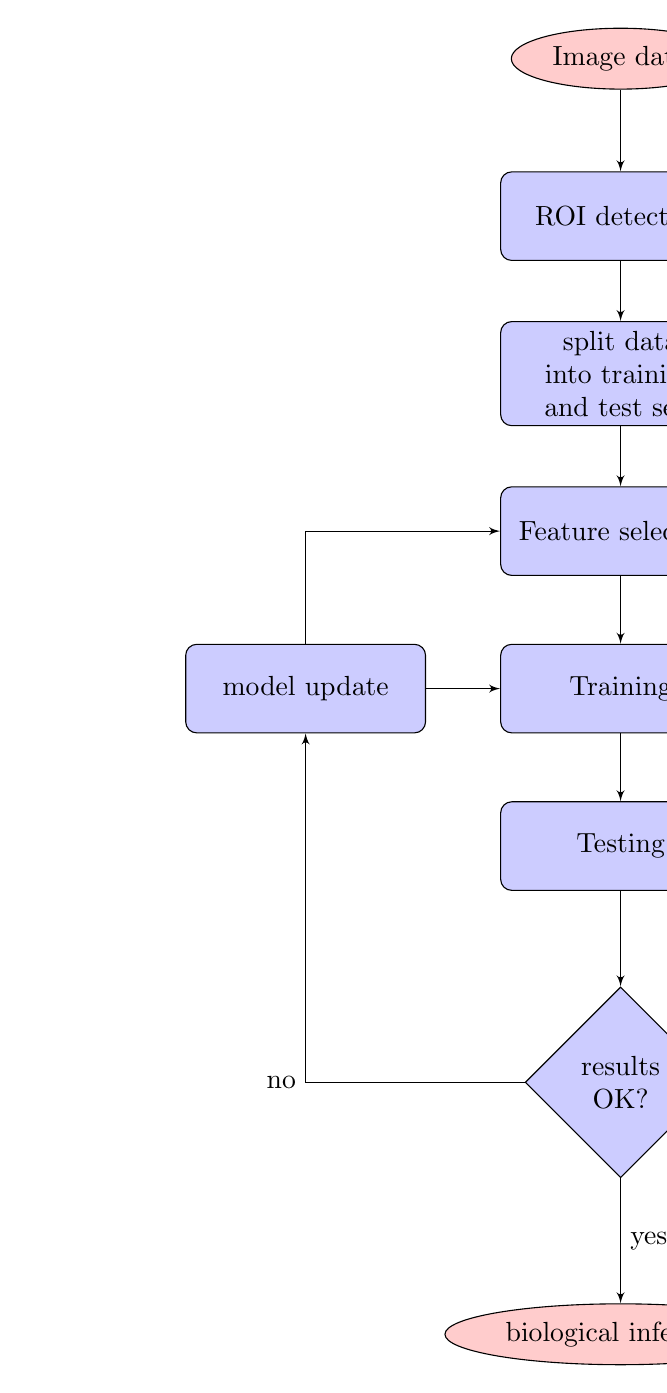
\begin{tikzpicture}[node distance = 2cm, auto]
    % Place nodes
    \node [cloud] (init) {Image data};
    \node [block, below of=init] (ROI) {ROI detection};
    \node [block, below of=ROI] (spl) {split data into training and test sets};
    \node [block, below of=spl] (ft) {Feature selection};
    \node [block, below of=ft] (train) {Training};
    \node [block, left of=train, node distance=4cm] (update) {model update};
    \node [block, below of=train] (test) {Testing};
    \node [decision, below of=test] (decide) {results OK?};
    \node [cloud, below of=decide, node distance=3.2cm] (stop) {biological inference};
    % Draw edges
    \path [line] (init) -- (ROI);
    \path [line] (ROI) -- (spl);
    \path [line] (spl) -- (ft);
    \path [line] (ft) -- (train);
    \path [line] (train) -- (test);
    \path [line] (test) -- (decide);
%     
    \path [line] (decide) -| node {no} (update);
    \path [line] (decide) -- node {yes}(stop);
    \path [line] (update) |- (ft);
    \path [line] (update) -- (train);

\end{tikzpicture}


\caption{Flowchart of Detection Algorithm}
\label{ch3:fig1}
\end{figure}


% \vspace{0.5cm}

\section{Definition of Classification}
\label{ch3:class}

In \Gls{ML} the idea of \textit{classification} refers to the problem of identifying to which of a set of categories
(named \textit{classe}s) a new observation belongs, on the basis of a training set of data containing instances whose category membership is known.
In case of mitosis detection, the elements of a classification are basically the following:

\begin{itemize}
\item the \textit{input} to the classification problem is a set of \textit{features} computed on each of the \textit{candidates} selected in a preparatory phase.
    Each set of features composing a candidate is known as \textit{instance}. Each instance is \textit{labeled}  with the \textit{class} which it belongs to.
\item the \textit{classes} are simply two: \texttt{mitosis} (which we call \textit{class 1} or \textit{positive})
    or \texttt{non-mitosis} (which we call \textit{class 0} or \textit{negative}) making it a case of binary classification.
\item the \textit{output} of the classification can be a \textit{hard} classification: the output of the classifier is simply \textit{0} or \textit{1},
    corresponding to mitosis or non-mitosis respectively. On the other hand the classification can be \textit{soft}: the output of the classifier is a real number \textit{c}:

\begin{equation}
 0 \leq c \leq 1
\end{equation}
a subsequent phase of analysis consists in selecting the best threshold so that:

\begin{equation}
   \textit{class}=\begin{cases}
    0, & \text{if $c<threshold$}.\\
    1, & \text{otherwise}.
  \end{cases}
\end{equation}
the selection of the threshold is made in function of the measured performances of the classification algorithm (see \ref{ch3:perf}).

\end{itemize}

\vspace{0.5cm}

\section{Review of Algorithms solving the mitosis detection problem}
\label{ch3:review}

Different to other pattern recognition tasks, mitotic cells essentially are irregular shape objects. As a result, there
is no simple or unique way of extracting the features of mitotic cells and then many different classifiers can be made.

Here we briefly review the main algorithms found in literature that solve the mitosis detection task.

\begin{itemize}
 \item[-] The method proposed in \cite{Mitosis01} consists of two main components: candidate extraction and candidate classification.
Candidate objects are extracted by image segmentation with the Chan-Vese level set method \cite{moelich2003tracking}.
A statistical classifier is trained with a number of features that describe the size, shape, color and texture of the candidate objects.
 \item[-] The approach in \cite{mitosisDetectBreastCancer01} uses, after a phase of automatic segmentation of the image, a \Gls{GGMM} to classify
the candidates: the \Gls{GGMM} is a parametric technique for estimating probability density function. In this context, it is formulated as a function of pixel intensities.
 \item[-] The work in \cite{breastCancerMitosisPCA_ICA} also proposes a two phases approach: the detection candidates points are selected by using
an algorithm named eXclusive Independent Component Analysis (XICA), which gives two sets of training patterns: positive and negative patterns (positive and negative basis set).
Then a sparse representation method \cite{wright2009robust} is used to classify the candidates.
 \item[-] Also the approach in \cite{irshad2011automated} has two phases.
In the first stage, the detection of candidate mitosis is performed. The input RGB
images are transformed into blue-ratio images. A Laplacian of Gaussian (LoG), thresholding and morphological operations on blue-ratio images is then executed 
to generate candidate mitosis regions. Then, the candidate regions are selected using morphological rules; the center point of each region is used  as seed point for mitosis.
In the second stage, co-occurrence features, run-length features and SIFT features are computed for each candidate patch.
Finally a classification is performed to put the candidate patch either in the mitosis class or in the non-mitosis class.
Three different classifiers have been evaluated: decision tree, linear kernel \Gls{SVM} and non-linear kernel \Gls{SVM}.
 \item[-] The article in \cite{mitoticRecognition03Agreement} uses a simple rule that extracts blobs representing nuclei of possible mitotic figures to establish a set of
candidates. \Gls{ML} is applied in three phases. One phase applies a support vector regression which remaps the color palette of the original image to
normalized values. The next phase is a \Gls{CNN}, applied at each extracted blob. The \Gls{CNN} contributes a generate a feature vector, which also contains many other
measurements regarding the shape, color, mass, and texture of the blob and its neighborhood. In the final phase, a \Gls{SVM} uses the feature vector to
classify the area around the blob as a mitotic figure or not.
\end{itemize}


The last two works that we mention here are particularly interesting because they work on the same dataset that we used, the \textit{MITOS Dataset} (see Chapter \ref{chapter4} for details).

\begin{itemize}
\item[-] The approach in \cite{irshad2013multispectral} works on z-stack focus planes for detection of mitosis candidates.
Then candidates are detected using thresholding and morphological operations on selected band and focus plane.
A multi-spectral features vector is computed for detected candidates having intensity and texture features across all bands
of multi-spectral images. In addition, using segmented regions of detected candidates, morphological features are also computed. A feature selection algorithm
is employed on this features vector in order to save the computation
cost, to discard any redundancy in the data, and to improve classification accuracy.
Classification is achieved using Bayesian, Decision Tree , Neural Network as
well as linear and non-linear \Gls{SVM} classifiers.
 \item[-] The approach in \cite{agNN} is procedurally simpler than other methods, as no candidate selection is performed.A supervised \Gls{DNN} as a powerful pixel classifier.
The \Gls{DNN} is a type of \Gls{CNN}. It directly operates on raw RGB data sampled from a square patch of the source image, centered on the pixel itself. The \Gls{DNN} is trained to
differentiate patches with a mitotic nucleus close to the center from all other windows.
Mitosis in unseen images are detected by applying the classifier on a sliding window, and post-processing its outputs with simple techniques. Because the \Gls{DNN} operates on
raw pixel values, no human input is needed.
\end{itemize}
 
In our work, we also used, as a reference, the performances other top-scoring algorithms developed for the \textit{MITOS Dataset}, whose main features will be described in
a special issue of the \textit{Journal of Pathology Informatics}\footnote{\url{http://www.jpathinformatics.org/}} expected for June 2013.


\vspace{0.5cm}


\section{Performance and Benchmarking}
\label{ch3:perf}

In order to set up a correct and valid comparison among mitosis detection algorithms, a consistent definition of \textit{performance} plays a fundamental role.
The general appearance of a mitosis results in the fact that automatically detecting mitoses is very challenging, and in fact even the agreement between pathologists is not perfect.

\vspace{0.5cm}

\subsection{Pathologists' Agreement}
\label{ch3:humans}

The work in \cite{mitoticRecognition03Agreement} deeply analyzes the agreement among pathologists examining the same \Gls{HE} images. The \Gls{BR} grading system is widely
recognized as the one giving the most stable definitions, and its grades are widely used to select treatments. Nevertheless, the level of agreement is shown to be far from perfect.

The level of agreement may be reported in Cohen's Kappa ($\kappa$) \cite{cohen1960coefficient} whose range is $0 \leq \kappa \leq 1$, with
\textit{\textbf{1}} corresponding to perfect agreement, and \textit{\textbf{0}} in the case of probabilistically independent decisions.\\

The value of $\kappa$ can be divided in ranges:

\begin{itemize}
 \item [-] \textbf{0-0.2} is often considered as \textit{slight} agreement,
 \item [-] \textbf{0.2–0.4} as \textit{fair},
 \item [-] \textbf{0.4–0.6} as \textit{moderate},
 \item [-] \textbf{0.6–0.8} as \textit{good},
 \item [-] \textbf{0.8–1} as almost \textit{perfect}.
\end{itemize}

Most studies show that value of $\kappa$ generally varies from \textit{fair} to \textit{moderate} (e.g. the study in \cite{meyer2005breast} reports a value of $\kappa = 0.5$).\\
The low level of agreement among pathologists is an issue also for algorithms' benchmarking, as it can be difficult to establish a definite \Gls{GT} (i.e. the process of gathering the proper objective data for the test).\\
Nonetheless, the images of the \textit{MITOS Dataset} have been annotated by only one pathologist: the algorithms of the \textit{2012 ICPR Contest} and our work based their \Gls{GT} on that.

\vspace{0.5cm}

\subsection{Benchmarking}
\label{ch3:bench}

Benchmarking of different algorithms and comparison with human performance play a key role in a detection framework, it is so of great importance the definition of \textit{performance}.\\
Given a \Gls{GT}, the \textit{Confusion Matrix} (or Error Matrix \cite{stehman1997selecting}), is so defined:
each column of the matrix represents the instances in a predicted class, while each row represents the instances in an actual class.
The name originates from the fact that it makes it easy to see if the system is confusing two classes (i.e. mislabeling one as another).
The elements of the matrix are:
\begin{itemize}
 \item [-] \textbf{TP}: \textit{True Positive}, a sample labeled as true is predicted as true,
 \item [-] \textbf{TN}: \textit{True Negative}, a sample labeled as false is predicted as false,
 \item [-] \textbf{FP}: \textit{False Positive}, a sample labeled as false is predicted as true (i.e. false alarm, or \textit{Type I} error),
 \item [-] \textbf{FN}: \textit{False Negative}, a sample labeled as true is predicted as false (i.e. miss, or \textit{Type II} error),
\end{itemize}


\begin{table}[!hbt]
 \caption{Confusion Matrix}
 \centering
 \begin{tabularx}{210pt}{ >{\centering\arraybackslash} X |>{\centering\arraybackslash} X |>{\centering\arraybackslash} X }
   & predicted \textit{Positive} & predicted \textit{Negative} \\
   \hline
   Actual \textit{Positive} & \cellcolor{YellowGreen}True Positive  & \cellcolor{OrangeRed}False Negative \\
                            & \cellcolor{YellowGreen} \text{(TP)} & \cellcolor{OrangeRed} \text{(FN)} \\
   \hline
   Actual \textit{Negative} & \cellcolor{OrangeRed}False Positive & \cellcolor{YellowGreen}True Negative \\
                            & \cellcolor{OrangeRed} \text{(FP)} & \cellcolor{YellowGreen} \text{(TN)} \\
  \hline
 \end{tabularx}
 \label{ch3:tab1}
\end{table}

The data in Table \ref{ch3:tab1} represent the minimum required data to assess the performance of a classifier (human or automatic).
Starting from this, some other measurements can be done.\\
The data in the table can be assembled to define some performance indicators.

\vspace{0.5cm}

\subsubsection{Accuracy}

The accuracy of a test represents the degree of closeness of prediction to the actual value, and it is measured as:

\begin{eqnarray}
 \textrm{Accuracy} \quad ACC & = & \frac{TP+TN}{P+N} \\
 \textrm{where} \quad P & = & TP + FN \ \textrm{and} \ N = TN + FP
\end{eqnarray}


\vspace{0.5cm}

\subsubsection{Precision, Recall, F-Score}

A first set of measures that can be done on the data of the confusion matrix are: \textit{precision},also named Positive Predictive Value (PPV),
\textit{recall}, or True Positive Rate (TPR), and \textit{F-Score} \cite{Precision_Recall_Fscore}.
They are defined as follows:

\begin{eqnarray}
 \textrm{Precision} \quad p & = & \frac{TP}{TP+FP} \\
 \textrm{Recall} \quad r & = &   \frac{TP}{TP+FN}
\end{eqnarray}

Both precision and recall have a natural interpretation in terms of probability. Precision may be defined as the probability that an instance
has class \textbf{1}, given that it is classified as \textbf{1}, while the recall is the probability that a class \textbf{1} object is classified:

\begin{eqnarray}
 p & = & P(\textrm{label} = true \mid \textrm{class} = true ) \\
 r & = & P(\textrm{class} = true \mid \textrm{label} = true )
\end{eqnarray}

The weighted (with parameter $\beta$) harmonic average of \textit{precision} and \textit{recall} leads to the \textit{F-Score}\cite{InfoRetrieval}:

\begin{equation}
 \textrm{F-Score} \quad F_{\beta} =  (1+\beta^{2}) \cdot \frac{pr}{r + \beta^{2}p} = \frac{(1+\beta^{2})TP}{(1+\beta^{2})TP + \beta^{2}FN + FP}
\end{equation}

$F_1$-Score is most widely used as a measure of the accuracy of the classifier.
It can be interpreted as a weighted average of the precision and recall: an $F_1$-Score reaches its best value at \textbf{1} and worst score at \textbf{0}.

\vspace{0.5cm}

\subsubsection{Specificity, Sensitivity}

\textit{Sensitivity} and \textit{Specificity} are often used in clinical tests as a measure of the ability of the test to confirm or 
refute the presence of a disease\cite{sensSpec}.
Ideally a test correctly identifies all patients with the disease, and similarly correctly identifies all patients who are
disease free. In other words, a perfect test is never positive in a patient who is disease free and is never negative in a patient who is in fact diseased.\\
The sensitivity of a clinical test refers to the ability of the test to correctly identify those patients with the disease:

\begin{equation}
 Sensitivity = \frac{TP}{TP + FN}
\end{equation}

It can be noted that the definition of sensitivity is the same as the definition of recall.
A high sensitivity is clearly important where the test is used to identify a serious but treatable disease.\\
The specificity, or True Negative Rate (TNR), of a clinical test refers to the ability of the test to correctly identify those patients without the disease:

\begin{equation}
 Specificity = \frac{TN}{TN + FP}
\end{equation}

High specificity results in few patients who are disease free being told of the possibility that they have the disease and are
then subject to further investigation or treatments. Also the following relation holds:

\begin{eqnarray}
 Specificity & = & 1 - FPR\\
 \textrm{where} \ FPR & = & \frac{FP}{FP + TN}
\end{eqnarray}

\vspace{0.5cm}

\subsubsection{Receiver Operating Characteristic (ROC)}
\label{ch3:roc}

As mentioned in \ref{ch3:class}, the classifier or diagnosis result can be a real value (continuous output),
in this case the boundary between the two classes of the binary classifier must be determined by a threshold value.
A \Gls{ROC} space is defined by FPR and TPR as \textit{x} and \textit{y} axes respectively, which depicts relative trade-offs between true positive (benefits) and false positive (costs)\cite{ROC01}.
Since TPR is equivalent with sensitivity and FPR is equal to 1 − specificity, the ROC graph is sometimes called the sensitivity vs (1 − specificity) plot\cite{ROC_precision_recall}.
Each prediction result or instance of a confusion matrix represents one point in the ROC space (see Figure \ref{ch3:fig2:a}).
The best possible prediction method would yield a point in the upper left corner or coordinate (0,1) of the ROC space, representing 100\% sensitivity (no false negatives)
and 100\% specificity (no false positives). The (0,1) point is also called a perfect classification. A completely random guess would give a point along a diagonal line
from the left bottom to the top right corners.\\
The diagonal divides the \Gls{ROC} space. Points above the diagonal represent good classification results (better than random),
points below the line poor results (worse than random).

\begin{figure}[!hbt]
  \centering
    \subfigure[ROC curve]{
      \includegraphics[width=0.84\textwidth]{./images/ROC1.png}
      \label{ch3:fig2:a}
    }\\
    %\hspace{1mm}
    \subfigure[AUC]{
      \includegraphics[width=0.84\textwidth]{./images/ROC2.png}
      \label{ch3:fig2:b}
    }
    \caption{Example of ROC curves}
    \label{ch3:fig2}
\end{figure}


The \Gls{ROC} is used to generate summary statistics. One of the often used is the area under the \Gls{ROC} curve, or \textit{AUC} (Area Under Curve)\cite{Brown200624, ROC02} (see Figure \ref{ch3:fig2:b}):
AUC is equal to the probability that a classifier will rank a randomly chosen positive instance higher than a randomly chosen negative one. The AUC can be related to other
summary statistics like the \textit{Gini coefficient} \cite{Gini} and the \textit{Mann-Withney U} \cite{MWU}.
Another common measure related to the \Gls{ROC} curve is known as the Area Under the ROC Convex Hull (\textit{AUCH ROC}, in Figure \ref{ch3:fig2:b}), which computes the area unter the convex hull of the ROC curve, as
it can be shown that any point on the line segment between two prediction results can be achieved by randomly using one or other system with probabilities proportional to the relative length of the opposite component of the segment.














% Impostazione del problema, modello
% - come si e' passati dal problema di detection al problema di classificazione
% - definizione del problema di classificazione, input, output, classi
% - come si affronta il problema di classificazione
% -- da un algoritmo (calcolo features, classificazione tramite classificatore)
% -- da un umano
% - defininzione di performance



\chapter{Design of a Mitosis Detection algorithm}
\label{chapter4}
\thispagestyle{empty}

\begin{quotation}
{\footnotesize
\noindent \emph{\textquotedblleft Ab uno\\ disces omnis\textquotedblright}\\
\noindent (Learn everything from one)
\begin{flushright}
Publius Vergilius Maro (Aeneis II, 65-66)
\end{flushright}
}
\end{quotation}

\vspace{0.5cm}

%\noindent In questa sezione si spiega come \`e stato affrontato il problema concettualmente, la soluzione logica che ne \`e seguita senza la documentazione.

We developed an algorithm to perform mitosis-detection as a part of our work, with the aim to compare its results with humans facing the same task.

\section{Dataset}
\label{ch4:ds}

We used the public MITOS dataset \cite{icpr}. The dataset is composed by a total of 50 2084$\times$2084 pixel images
covering an area of 512$\times$512 $\mu$m each, acquired with an APERIO XT scanner (see Figure \ref{ch2:fig1}). 
A unique split is defined by the dataset authors, with 35 images used for training and 15 for evaluation.
The dataset contains a total of about 300 mitosis, which were annotated by an expert pathologist.
The performance of the algorithms participating to the \textit{2012 ICPR mitosis detection contest} are shown in Section \ref{ch3:icpr_perf}.\\
With reference to Figure \ref{ch3:fig1}, we focused on on the classification subproblem, with the \Glspl{ROI} given as an input.
The input is given in form of an image patch with size 100$\times$100 pixel: such size completely contains the image of the cell.
The task is to map each patch to one of two classes:
\begin{itemize}
 \item [] \textit{\textbf{C1}}: the image contains a mitosis at its center,
 \item [] \textit{\textbf{C0}}: the image does not contain a mitosis anywhere. 
\end{itemize}

There are no samples in which a mitosis is visible off-center.

\vspace{0.5cm}

\subsection{Image Candidates}
\label{ch4:ic}

For the \textit{\textbf{C1}} class, all the 216 mitosis available in the 35 training images are chosen
as training samples, and all 87 mitosis in the evaluation images are chosen as
evaluation samples.\\
We enforced an even distribution of the two classes classes both in training and in evaluation sets, and therefore
selected 216 \textit{\textbf{C0}} samples for training, and 87 \textit{\textbf{C0}} samples for evaluation; the resulting
training set contained 432 samples.\\
Millions of different \textit{\textbf{C0}} samples may be randomly chosen from the original training and evaluation images:
an overwhelming majority of such samples would not contain any nucleus and be non-informative for training and trivial for
evaluation. Limiting the choice to non-mitotic nuclei \texttwelveudash{} which greatly outnumber
mitotic ones \texttwelveudash{} would not solve the problem, since most of such nuclei look very
similar to each other and are trivially identified as non-mitotic. Only a small
subset of non-mitotic nuclei \texttwelveudash{} as well as other structures and artifacts \texttwelveudash{} pose an
actual challenge, both for humans and for algorithms.\\
In order to select such objects as \textit{\textbf{C0}} samples, we used the output produced by a simple \Gls{CNN}-based mitosis detector,
similar to the one outlined in \cite{agNN} for selecting useful training samples.
The detector, built at IDSIA, was trained on few images in the training set, then applied on the whole dataset.
Because the detector was simple and trained on a small amount of data, it performed poorly and detected a lot of false positives.
\textit{\textbf{C0}} samples have been randomly chosen among the outputs of such detector which are
farther than 50 pixels from the centroid of any mitosis; this ensures that no actual
mitosis is visible in the corresponding image patch. The resulting samples do in
fact resemble mitosis, are informative in the training set, and appear non-trivial
in the evaluation set. Finally, 10 \textit{\textbf{C0}} samples in the evaluation set are substituted
with 5 random false positives obtained from each of the two best performing
algorithms (IDSIA and IPAL). These last 10 samples are particularly useful to compare humans to algorithms, in fact allowed us to better observe how test subjects
behave on the algorithms’ false positives, which are rare in the evaluation set because
algorithms were tuned to solve a problem with very low prevalence of mitotic samples.


\vspace{0.5cm}

\subsection{Extended Dataset}
\label{ch4:ed}

We extended our dataset by rotating and mirroring each image patch (see Figure \ref{ch4:fig1}). We used the extended dataset only for the detection algorithm, so that we could analyze
the effect of different features, which can be explicitly dependent on orientation or not, on the global performance of the classifier.\\
In case of extended dataset, the classification of a single image patch becomes the average of the classifications obtained on the 8 samples.

\begin{equation}
 c_{i} = \frac{\sum_{j=1}^{8} c_{ij}}{8}
\end{equation}

Where $c_{i}$ represents the classification of image patch \textit{i}, and $c_{ij}$ represents the classification of variation \textit{j} of image patch \textit{i} .



\begin{figure}[!hbt]
  \centering
    \includegraphics[width=0.94\textwidth]{./images/rotDataset.png}
  \caption[Extended Dataset]{Extended dataset\\(a),(b),(c): $\pi/2$ clockwise rotations, (d),(e),(f): mirror and $\pi/2$ clockwise rotations.}
  \label{ch4:fig1}
\end{figure}  

\vspace{0.5cm}




\section{Feature Extraction}
\label{ch4:FE}

Each image patch can be represented as a 100$\times$100$\times$3 matrix, where the $(i,j,:)$ triplet represents the RGB value of point with coordinates $(i,j)$ in the image.
Each value is in the range 0 to 255. Starting from these (raw) data we extracted some features by which we trained and tested our classifiers.

\vspace{0.5cm}

\subsection{Simple Features}
\label{ch4:sf}

The simplest features that can be computed involve the average and the standard deviation of the \Gls{RGB} values of the image patch. They can be computed on all the data or can be maintained separated
for each \Gls{RGB} component. In the first case, average and standard deviation each give one value every instance:

\begin{eqnarray}
 m & = & \frac{1}{100\cdot100\cdot3} \left( \sum_{i=1}^{100} \sum_{j=1}^{100} \sum_{k=1}^{3} i_{ijk} \right) \\
 \sigma & = & \sqrt{\frac{1}{100\cdot100\cdot3} \left( \sum_{i=1}^{100} \sum_{j=1}^{100} \sum_{k=1}^{3} (i_{ijk} - m )^2 \right)}
\end{eqnarray}

Otherwise, average and standard deviation produce a vector of three components:

\begin{eqnarray}
 \overline{M} & = & \left[ \begin{array}{c}
                            \frac{1}{100\cdot100} \left( \sum_{i=1}^{100} \sum_{j=1}^{100} i_{ij1} \right) \\
                            \frac{1}{100\cdot100} \left( \sum_{i=1}^{100} \sum_{j=1}^{100} i_{ij2} \right) \\
                            \frac{1}{100\cdot100} \left( \sum_{i=1}^{100} \sum_{j=1}^{100} i_{ij3} \right)
                           \end{array} \right] \\
 \overline{S} & = & \left[ \begin{array}{c}
                                 \sqrt{\frac{1}{100\cdot100} \left( \sum_{i=1}^{100} \sum_{j=1}^{100} (i_{ij1} - M(1) )^2 \right)} \\
                                 \sqrt{\frac{1}{100\cdot100} \left( \sum_{i=1}^{100} \sum_{j=1}^{100} (i_{ij2} - M(2) )^2 \right)} \\
                                 \sqrt{\frac{1}{100\cdot100} \left( \sum_{i=1}^{100} \sum_{j=1}^{100} (i_{ij3} - M(3) )^2 \right)}
                                \end{array}  \right]
\end{eqnarray}

Another simple set of features is represented by the \textit{median} of each \Gls{RGB} value. The median is defined as the numerical value separating the higher half of the data sample, from the lower half
and can be found by arranging all the data from lowest value to highest value and picking the middle one, or the mean of the two middle values, in case of even data.
Each of the features above are independent of the orientation of the image.
%	-	m: mean
%	-	s: standard deviation
%	-	M: mean per color
%	-	S: std per color
%	-	d: median per color



\vspace{0.5cm}

\subsection{Color Histograms and Intensities}
\label{ch4:chi}

A color histogram is a representation of the distribution of colors in an image, i.e. the number of pixels that have colors in each of a fixed list of color ranges \cite{colorHistogram01},
that span the image's color space. The color histogram can be built for any kind of color space, although the term is more often used for three-dimensional spaces like \Gls{RGB} or \Gls{HSV}.
A histogram of an image is produced first by discretization of the colors in the image into a number of bins, and counting the number of image pixels in each bin.
We built the \Gls{RGB} color histogram for each image patch, using 16 bins for each channel. The feature vector is so composed of 48 elements.\\
Also this feature is orientation independent.


\begin{figure}[!hbt]
  \centering
    \includegraphics[width=0.94\textwidth]{./images/histIM.png}
  \caption[Color Histograms]{Color Histograms of sample image}
  \label{ch4:fig2}
\end{figure}  

It is generally possible to transform a color image into a gray-scale one. One typical transformation algorithm, applied pixel by pixel, is the following:

\begin{equation}
 \label{ch4:eqGS}
 pix_{gray} = 0.2989 \cdot pix_{red} + 0.5870 \cdot pix_{green} + 0.1140 \cdot pix_{blue}
\end{equation}

On the resulting monochromatic image, it is possible to compute an \textit{intensity histogram}.\\
We preferred to compute a slightly different feature: the average intensity in the 25 central regions of the image.
We first computed the gray-scale image according to Equation \ref{ch4:eqGS}, then we selected the central part of the image and divided it in a grid of $5\times5$ elements.
We finally computed the mean intensity for each element. Figure \ref{ch4:fig3} illustrates the procedure.

\begin{figure}[!hbt]
  \centering
    \includegraphics[width=0.94\textwidth]{./images/GSintens1.png}
  \caption[Example of mean gray-scale intensities feature]{Mean gray-scale intensity of central part of image patch}
  \label{ch4:fig3}
\end{figure}

The resulting feature vector is composed of 25 values, corresponding to the intensities, ordered columnwise. This type of feature is orientation dependent.

%	-	H: color histograms (16 bins)
%	-	i: mean intensity in 25 central regions of the image


\vspace{0.5cm}

\subsection{Texture Features}
\label{ch4:tf}

Texture features are widely used in different \Gls{CV} tasks, as pointed out in Section \ref{ch2:texture}. We focused on the features described in \cite{LBP01} and \cite{LBP02},
based on Local Binary Patterns (\Gls{LBP}). The general idea of \Gls{LBP} is described on page \pageref{ch2:lbp}.
The \Gls{LBP} features considered here are labeled LBP$_{P,R}$, where \textit{P} is the number of neighbors considered and \textit{R} is the distance from the pixel.
The two main characteristics of the \Glspl{LBP} considered are:

\begin{itemize}
 \item \textit{uniformity}: which is a fundamental property of local image texture. It refers to the uniform appearance of the local
binary pattern, that is, there is a limited number of transitions or discontinuities in the circular presentation of the pattern.
The most frequent uniform binary patterns correspond to primitive \textquotedblleft microfeatures\textquotedblright, such
as edges, corners, and spots; hence, they can be regarded as feature detectors that are triggered by the best matching
pattern.
\item \textit{rotation invariance}: which takes into account if a spatial pattern is affected by rotation or not.
\end{itemize}

Three different types of features can be built, on the basis of Equation \ref{ch2:eq_lbp1}:

\begin{enumerate}
 \item $\text{LBP}_{P,R}^{u2}$: uniform feature,
 \item $\text{LBP}_{P,R}^{ri}$: rotation invariant feature,
 \item $\text{LBP}_{P,R}^{riu2}$: uniform and rotation invariant feature,
\end{enumerate}

In particular we used:

\begin{equation}
 \text{LBP}_{8,R}^{\text{type}} \quad \textrm{where} \begin{cases}
    \text{type}  & \in \{ri, u2, riu2\}\\
    R  & \in \{1,2,3\}
  \end{cases}
\end{equation}

while building the feature vector, we used the \textit{type} parameter in a mutually exclusive way, i.e. we did not concatenate \Glspl{LBP} of different types. On the other hand, we
built feature vectors with various combitations of radii.\\
The following equations show the three different mutually exclusive texture feature sets that we considered.

\begin{eqnarray}
\label{ch4:tftypes}
 \overline{L} & = & \left[ \text{LBP}_{8,1}^{riu2}, \text{LBP}_{8,2}^{riu2}, \text{LBP}_{8,3}^{riu2} \right] \\
 \overline{U} & = & \left[ \text{LBP}_{8,1}^{u2}, \text{LBP}_{8,2}^{u2}, \text{LBP}_{8,3}^{u2} \right] \\
 \overline{R} & = & \left[ \text{LBP}_{8,1}^{ri}, \text{LBP}_{8,2}^{ri}, \text{LBP}_{8,3}^{ri} \right]
\end{eqnarray}

Finally, we considered the \Gls{VAR} operator, as described in Equation \ref{ch2:eq_lbp2}. As, from early tests, a single \Gls{VAR} value for the entire image patch proved to be non-significant, we
decided to follow an approach similar to the one described for the intensity histogram (see Figure \ref{ch4:fig3}) and evaluated the mean value of a grid of samples in the central
region of the image. Figure \ref{ch4:fig4} shows a sample of $VAR(8,1)$ computation. Please note that the gray-scale mapping of the VAR(8,1) figure has been adjusted to be visible with full gray-scale range.

\begin{figure}[!hbt]
  \centering
    \includegraphics[width=0.94\textwidth]{./images/GS_VAR.png}
  \caption[Example of VAR(8,1) feature]{Example of VAR(8,1) feature}
  \label{ch4:fig4}
\end{figure}

The resulting feature vector is composed of 36 values, corresponding to the average VAR(8,1) in each element of the grid, ordered columnwise. This type of feature is orientation dependent.
\\
The Matlab code implemented to build the feature vectors is listed in \ref{appendixB:FE}


% \clearpage

%	-	l: lbp riu2 radius 1, 8 neighbors
%	-	r: lbp ri radius 1, 8 neighbors
%	-	u: lbp u2 radius 1, 8 neighbors
%	-	v: mean pixel variance
%	-	L: lbp riu2 radius 1-2-3, 8 neighbors concatenated
%	-	V: pixel variance, 36 elements
%	-	R: lbp ri radii 1-2-3, 8 neighbors
%	-	U: lbp u2 radii 1-2-3, 8 neighbors



\vspace{0.5cm}

%\clearpage

\section{Classifiers}
\label{ch4:classifiers}

Once defined the set of feature to be considered, it is possible to build a matrix whose lines represent an \textit{instance} (i.e. an image patch) and whose columns represent a \textit{feature}
(or a component of it): Equation \ref{ch4:fmat} represents such matrix.
\begin{equation}
\label{ch4:fmat}
 M_{feats} = \\ \bordermatrix{~ & \tikzmark{harrowleft} 1 & \cdots & ~  & \cdots & ~ & \cdots & ~ & n_{fc}\tikzmark{harrowright}  \cr
			      \tikzmark{varrowtop} 1 & c_{111} & c_{112} & \cdots & c_{1k1} & \cdots & c_{1kn_k} & \cdots & c_{1n_f1} \cr
			                      \vdots &    ~    &   ~     &   ~    &    ~    &   ~    &     ~     &    ~   &     ~     \cr
			                       ~     & \vdots  & \vdots  & \ddots & \vdots  & \ddots & \vdots    & \ddots &  \vdots   \cr
			                      \vdots &    ~    &   ~     &   ~    &   ~     &   ~    &    ~      &    ~   &    ~      \cr
			      \tikzmark{varrowbottom} n_i & \tikzmark{f1} c_{n_i11} & c_{n_i12} \tikzmark{f2} & \cdots & \tikzmark{f3} c_{n_ij1} & \cdots & c_{n_ijn_j} \tikzmark{f4} & \cdots & \tikzmark{f5} c_{n_in_f1} \tikzmark{f6} \cr
			     }
\end{equation}
\tikz[overlay,remember picture] {
  \draw[->] ([yshift=3ex]harrowleft) -- ([yshift=3ex]harrowright)
            node[midway,above] {\tiny \textit{features}};
  \draw[->] ([yshift=1.5ex,xshift=-0.8ex]varrowtop) -- ([xshift=-0.8ex]varrowbottom)
            node[pos=0.0,anchor=north,xshift=-0.65cm,yshift=-2.3cm] {\tiny \textit{instances}};
  \draw [thick, decoration={ brace, amplitude=8pt, mirror, raise=0.12cm}, decorate] (f1) -- (f2) 
	    node [pos=0.5,anchor=north,yshift=-0.36cm] {\tiny \textit{feat$_1$}};
  \draw [thick, decoration={ brace, amplitude=8pt, mirror, raise=0.12cm}, decorate] (f3) -- (f4) 
	    node [pos=0.5,anchor=north,yshift=-0.36cm] {\tiny \textit{feat$_j$}};
  \draw [thick, decoration={ brace, amplitude=5pt, mirror, raise=0.12cm}, decorate] (f5) -- (f6) 
	    node [pos=0.5,anchor=north,yshift=-0.36cm] {\tiny \textit{feat$_{nf}$}};
}

Where $n_f$ is the total number of features and $n_i$ is the total number of instances. Each feature can be made of more than one component (e.g. $feat_1$ and $feat_j$ in the example).
For this reason, the total number of columns in the matrix $(n_{fc})$ is given by the sum of all the feature components. So, 
each element of the matrix $c_{ijk}$ is the $k^{th}$ component of the $j^{th}$ feature in the $i^{th}$ instance. The matrix representing the eavluation set is built in the same way.\\
A vector represents the class which every instance belongs to. Equation \ref{ch4:cvect} describes such vector:
\begin{equation}
\label{ch4:cvect}
 V_{class} = \\ \bordermatrix{~ &  ~  \cr
			      \tikzmark{varrowtop} 1 &  \tikzmark{f5} e_{1}  \tikzmark{f6} \cr
			                      \vdots & \vdots \cr
			                       ~     & e_i   \cr
			                      \vdots & \vdots \cr
			      \tikzmark{varrowbottom} n_i & e_{n_i} \cr
			     }
\end{equation}
\tikz[overlay,remember picture] {
  \draw[->] ([yshift=1.5ex,xshift=-0.8ex]varrowtop) -- ([xshift=-0.8ex]varrowbottom)
            node[pos=0.0,anchor=north,xshift=-0.65cm,yshift=-2.3cm] {\tiny \textit{instances}};
  \draw [thick, decoration={ brace, amplitude=3pt, raise=0.25cm}, decorate] (f5) -- (f6) 
	    node [pos=0.5,anchor=north,yshift=0.76cm] {\tiny \textit{class}};
}

where $e_i$ belongs to one of the two classes. In some implementations of binary classifiers it is required that $e_i \ \in \{-1,1\} \ \forall i = 1,\cdots,n_i$,
otherwise $e_i \ \in \{0,1\} \ \forall i = 1,\cdots,n_i$. The vector 
representing the \Gls{GT} of the evaluation set is built in the same way.\\
Having a matrix representing the training feature set, a matrix representing the evaluation (i.e. testing) feature set and two vectors including the \Gls{GT}
classification of each image patch, it is possible to run a classifier that tries to get insights form the feature set in order to classify the evaluation set.\\


In our work we focused on two types of classifiers:

\begin{itemize}
 \item \textit{Support Vector Machines}, which are widely used in computer vision classification problems, in particular
in biomedical imaging (\cite{mitosisDetectionLearningBased, SVM02, SVM03, SVMClassHistogram}, see also Section \ref{ch3:review}),
 \item \textit{Random Forests}, which is a relatively new ensemble approach that can also be thought of as a form of nearest neighbor predictor (\cite{randForests03,randForests02,randForests04}).
\end{itemize}

We also mention \Gls{CNN}, as it played a relevant role in the definition of our dataset (see Section \ref{ch4:ic}).


\vspace{0.5cm}

\subsection{Support Vector Machines}
\label{ch4:svm}

We used the Matlab implementation of the \textit{libSVM} described in \cite{SVM01}. \Glspl{SVM} are a popular classification technique.
The goal of \Gls{SVM} is to produce a model (based on the training data) which predicts the target values of the test data
given only the test data attributes. Given a training set of instance-label pairs $(\mathbf{x_i}, y_i)$, $i = 1,\cdots,l$, where $\mathbf{x_i} \in \mathbb{R}^n$ and $y \in \{-1,1\}^l$.\\
The \Gls{SVM} requires the solution of the following optimization problem:

\begin{equation}
     \begin{aligned}
      \smash{\min_{\textbf{w},b,\xi}} \quad & \frac{1}{2}\textbf{w}^T\textbf{w}+C \sum_{i=1}^{l}\xi_i   \\
      \text{Subject to:} &\\
       & y_i \left(\textbf{w}^T \phi( \mathbf{x_i} ) +b\right) \geq 1-\xi_i \\
       & \xi_i \geq 0 
     \end{aligned}
     \phantom{\hspace{3cm}} %%<---adjust the value as you want
\end{equation}

The training vectors $\mathbf{x_i}$ are mapped into a higher dimensional space (maybe infinite), by the function $\phi$.
\Gls{SVM} finds a linear separating hyperplane with the maximal margin in this higher dimensional space.
$C > 0$ is the penalty parameter of the error term.
The function

\begin{equation}
 K(\mathbf{x_i}, \mathbf{x_j}) = \phi(\mathbf{x_i})^T\phi(\mathbf{x_j})
\end{equation}

is called the \textit{kernel function}. Many kernel functions have been defined, the most common are:

\begin{itemize}
 \item \textit{linear}: $K(\mathbf{x_i}, \mathbf{x_j}) = \mathbf{x_i}^T\mathbf{x_j}$,
 \item \textit{polynomial}: $K(\mathbf{x_i}, \mathbf{x_j}) = \left(\gamma \mathbf{x_i}^T\mathbf{x_j} + r \right)^d, \gamma > 0$,
 \item \textit{\Gls{RBF}}: $K(\mathbf{x_i}, \mathbf{x_j}) = \exp{\left(-\gamma \lVert \mathbf{x_i} - \mathbf{x_j} \rVert^2 \right)}, \gamma > 0$,
 \item \textit{sigmoid}: $K(\mathbf{x_i}, \mathbf{x_j}) = \tanh \left( \mathbf{x_i}^T\mathbf{x_j} + r \right)$.
\end{itemize}

Where $\gamma$, \textit{d} and \textit{r} are kernel parameters \cite{ML01}.\\
In our work we focused on \Glspl{RBF} and sigmoid kernels, which are used in most cases.
In \Glspl{SVM} the \textit{support vectors} are the training instances that concur to define the separating hyperplane in the kernel space. The 
image of Figure \ref{ch4:fig5} gives a linear representation of a \Gls{SVM}.

\begin{figure}[!hbt]
  \centering
    \includegraphics[width=0.98\textwidth]{./images/SVM_example.png}
  \caption{Representation of a SVM}
  \label{ch4:fig5}
\end{figure}


\vspace{0.5cm}

\subsection{Random Forests}

\Glspl{DT} are attractive classifiers due to their high execution speed and simplicity. However, trees often suffer from performance loss, in terms
of generalization accuracy on unseen data when the complexity of the problem grows \cite{randForests01}.\\
Random Forests are a combination of tree predictors such that each tree depends on the values of a
random vector sampled independently and with the same distribution for all trees in the forest \cite{randForests03}.
So, \Gls{RF} can be viewed as an ensemble approach that can also be thought of as a form of nearest neighbor predictor.
Ensembles are a divide-and-conquer approach used to improve performance. The main principle behind ensemble methods is that a group of \textquotedblleft weak learners\textquotedblright
can be combined together to form a \textquotedblleft strong learner\textquotedblright. Each classifier, individually, is a weak learner, while all the classifiers taken together are a strong learner.
An example of \Gls{DT} is shown in Figure \ref{ch4:fig6}.

\begin{figure}[!hbt]
  \centering
    \includegraphics[width=0.98\textwidth]{./images/DT_example.png}
  \caption{Example of a Decision Tree}
  \label{ch4:fig6}
\end{figure}

A \Gls{RF} is composed by a number of trees \textbf{T}. For some number \textit{m}, \textit{m} features are randomly selected from the feature vector.
The subset of variables is used to train a \Gls{DT}.\\
According to Breiman implementation of \Glspl{RF}, \textit{m} should be that  $\ll$ than the number of features.\\
We adopted the convention in \cite{randForests03} that $m \leq \log_2 F +1$ and used an ensemble of 500 trees.\\
Running a \Gls{RF},when a new input is entered into the system (a test sample), it is run down all of the trees, each of which classifies
it in a \textquotedblleft hard\textquotedblright way (see \ref{ch3:class}): in a sense, each tree gives a vote for the current sample. 
The result is the average  of all of the terminal nodes that are reached, giving a final \textit{soft} classification.
\Glspl{RF} are generally quite fast, robust classifiers, and are also used in image classification \cite{randForests04}.
\\
The Matlab code implemented to classify data is listed in \ref{appendixB:Cl}.

\vspace{0.5cm}


\section{Classification Process}

Once a classifier is trained on the training set, it can be used to classify unseen data (i.e., the evaluation or testing set). The classifier
function is applied to each instance of the \textit{evaluation} feature set, which is built as the matrix described in Equation \ref{ch4:fmat}.\\
The output of the classifier is a vector like the one described in Equation \ref{ch4:cvect}, unless that, generally, the classification
process gives a \textit{soft} classification (see Section \ref{ch3:class}), which means that  $-1 \leq e_i \leq 1 \ \forall i = 1,\cdots,n_i$, or
$0 \leq e_i \leq 1$, depending on the definition of the classes.\\
The performance parameters are computed as a function of a \textit{classification threshold}, as described in Section \ref{ch3:roc}.



% In most computer vision applications it is not sufficient to extract only one type of feature to obtain the relevant information from the image data.
% Instead two or more different features are extracted, resulting in two or more feature descriptors at each image point.
% A common practice is to organize the information provided by all these descriptors as the elements of one single vector,
% commonly referred to as a feature vector. The set of all possible feature vectors constitutes a feature space.
% A common example of feature vectors appears when each image point is to be classified as belonging to a specific class.
% Assuming that each image point has a corresponding feature vector based on a suitable set of features,
% meaning that each class is well separated in the corresponding feature space, the classification of each image point can be done using standard classification method.

 



\chapter{Design of a User Study}
\label{chapter5}
\thispagestyle{empty}

\begin{quotation}
{\footnotesize
\noindent{\emph{``\greek{`p'antwn qrhm'atwn m'etron', >'anjrwpon e>~inai, 't~wn m`en >'ontwn <wc >'esti, t~wn d`e m`h >'ontwn <wc o>uk >'estinv.'}''}\\
(man is \textquotedblleft the measure of all things, of the existence of the things that are and the non-existence of the things that are not.\textquotedblright)}
\begin{flushright}
\greek{Pl'atwn}(Plato, Theaet. 152a)
\end{flushright}
}
\end{quotation}

% ὄντων ὡς ἔστι, τῶν δὲ μὴ ὄντων ὡς οὐκ ἔστιν.’

\vspace{0.5cm}

%\noindent Si mostra il progetto dell'architettura del sistema con i vari moduli.

\section{Test Design}

The problem of detecting mitosis can be cast as a problem of classifying image
patches. In fact, most detection algorithms are based on classifiers which map
an image patch to the probability that a mitosis appears at its center; once such
classifier is known, the detection problem is solved by applying it on a sliding
window over the input image, or to a set of candidate patches identified in a
previous step.
The classification task can be presented to an user through a very simple and immediate interaction mechanism: in fact, a single decision is required for each
patch. In contrast, detection would require a more complicated interaction with
users. For this reason, we focus on the classification subproblem in the following.
For a given sample, input is given in form of an image patch with size 100 × 100
px: such size completely contains the image of the cell, and most algorithms
(FIXME) considered in the following only use data from a smaller window. The
task is to map each patch to one of two classes: C1) the image contains a mitosis
at its center; C0) the image does not contain a mitosis anywhere. There are no
samples in which a mitosis is visible off-center.


\subsection{Dataset}

(NB: il set di immagini usate deve esser già stato descritto)

\subsection{User Interface}

Description of the website used to collect data from users.

\vspace{0.5cm}

\section{Data collection}

Description of the data collected by the website
\chapter{Experimental Results}
\label{chapter6}
\thispagestyle{empty}

\begin{quotation}
{\footnotesize
\noindent\emph{``Quote 6''}
\begin{flushright}
Author 6
\end{flushright}
}
\end{quotation}

\vspace{0.5cm}

%\noindent Si mostra il progetto dal punto di vista sperimentale, le cose materialmente realizzate. In questa sezione si mostrano le attivit\`a sperimentali svolte, si illustra il funzionamento del sistema (a grandi linee) e si spiegano i risultati ottenuti con la loro valutazione critica. Bisogna introdurre dati sulla complessit\`a degli algoritmi e valutare l'efficienza del sistema.

\section{Accuracy of the Detection Algorithm}

\vspace{0.5cm}

\section{Accuracy of Humans}

\vspace{0.5cm}

\section{Accuracy of Algorithms}

(rif. paper)
\chapter{Conclusions}
\label{chapter7}
\thispagestyle{empty}


\begin{quotation}
{\footnotesize
\noindent{\emph{``\greek{di`o o>ud'epote noe~i >'aveu fant'asmatoc <h yuq'h}''}\\
(The soul never thinks without a picture)}
\begin{flushright}
\greek{>Aristot'elhc} (Aristotle, On the Soul 4.7.431a16)
\end{flushright}
}
\end{quotation}

\vspace{0.5cm}


\section{Context and Results}

Breast cancer is one of the most deadly cancers for women. According to the increasing incidence rate of breast
cancer reported in many countries, early cancer detection and treatment play a major role
in increasing the chances of recovery from the disease. Nottingham Grading
System \Gls{NGS} is the standard grading procedures used in breast cancer assessment;
it focuses on three criteria: Mitotic Count , Nuclear Pleomorphism , and
Tubule Formation. Each criterion can be assigned with 3 scores, and the final
equivalent NGS grade is the summation of all three criteria.\\
Breast tissue samples of patients are taken for grading by means of biopsy. The \Gls{NGS} grade
of tissue samples are based on the deviation of the cell structures from normal
tissues.\\
Pathologists need to assess lots of tissue samples under the microscope every day.
Low agreement for medical cases is typical between pathologists
because they exam breast tissue samples based on their experience and opinion.
Hence, the evaluation of breast cancer grading is a subjective, manual, and
time-consuming process.\\
Digital high resolution histo-pathological images are commonly used for extracting useful structural information from samples
With the rapid growth in computer technologies, many computer science researches have
focused on computer aided diagnosis (\Gls{CAD}) systems to develop a standard and
quantitative measurement for breast cancer assessment.\\
From the application point of view, the most important issue is whether such algorithms
perform in such a way that can be compared to experts who routinely solve the same task.
In our work, we considered the perspective of the machine learning algorithm designer.
In this context, comparing an algorithm with an expert does not provide
much useful information, because they are not competing fairly. In fact, during
its formation and previous activity, the expert had access to an amount of training information (in form of criteria, guidelines and labeled examples) which is
most probably much larger than the algorithm's training set. So if a detection algorithm underperforms, when compared to a pathologist,
we can argue if it is due to its lack of detection ability (and then, effort should be
focused on improving it), or because it has not enough data to learn (which implies that effort should be instead focused on gathering larger labeled datasets).
We aimed to answer this question in the context of mitosis detection in breast
cancer histological images using the public MITOS dataset. 
We built a balanced dataset (50\% of mitoses and 50\% of non-mitoses) using all the labeled samples provided with the MITOS dataset (216 mitoses in the training set and 87 mitoses in
the evaluation set) and selected an equal number of negative samples which were not obviously non-mitoses.\\
We studied how top-performing algorithms in the recent ICPR2012 mitosis detection contest performed on the specific dataset. Furthermore 
we developed some detection algorithm using state of the art machine learning techniques.\\
We compared the results with the performance of humans which were new to the mitosis detection problem.
In order to do so, we designed an user test that placed such humans in the same conditions
as algorithms (i.e. they were provided with the same training data and tested
on the same evaluation data).\\
In this context, human performance represents as a lower bound on the performance of the ideal algorithm.\\
If we had observed that the best performing among such humans significantly outperforms an algorithm, we could
conclude that the algorithms lack either power or generalization ability, and
can therefore be improved. Otherwise, the algorithm's performance may only be
limited by the amount of available training data.\\
Our main contribution is an user study whose results provide strong evidence in favor of the second hypothesis : we found that the two top-scoring algorithms
and the best ones that we developed perform comparably or better than the top-scoring human who took our test, which suggests that training set size may be limiting
the performance of such algorithms.

\vspace{0.5cm}

\section{Future Work}

Our work focused on the comparison of the performance of humans and on algorithm from the classification point of view ( i.e. the image candidates were previously selected).
The whole process of mitotic count requires the detection of candidates and then classification. It would be interesting carry experiments on the detection phase,
comparing human ability to detection algorithms' performance.\\
Our work could be extended by selecting some histologists and let them classify our dataset. The results would be interesting from different viewpoints: on one side their results
can be compared to algorithms and other users, and gain some information on possible differences in the performances of the three sets. On the other side, as 
mitosis detection is widely recognized as a difficult problem, characterized by moderate agreement even among histologists, their results can be used to validate the quality of the 
dataset and in general to confirm the difficulty of the task.\\
A study similar to the one presented here could be carried out on a larger dataset, so that a comparison among algorithms and pathologists could give significant information: 
it could be possible to draw correlations among the errors of algorithms and humans and verify the accuracy of algorithms.\\
Finally, extending the test to histologist, could bring information on possible difference among different types of users. Non-expert users, being all trained in the same way,
tend to present the same errors, without specific biases. Nevertheless, they tend to be less accurate. Histologists, being trained at different times, in different ways and
maybe with different criteria, should reach great accuracy but could make different kind of errors, depending on their background.




%\noindent Si mostrano le prospettive future di ricerca nell'area dove si \`e svolto il lavoro. Talvolta questa sezione pu\`o essere l'ultima sottosezione della precedente. Nelle conclusioni si deve richiamare l'area, lo scopo della tesi, cosa \`e stato fatto,come si valuta quello che si \`e fatto e si enfatizzano le prospettive future per mostrare come andare avanti nell'area di studio.

\cleardoublepage
% ---- Bibliography ----

\backmatter

\addcontentsline{toc}{chapter}{Bibliography}
\bibliographystyle{acm}
\thispagestyle{empty}
\bibliography{Bibl_thesis}
%\nocite{*}

\appendix

\pagestyle{fancy} 
\fancyfoot{}                                               
\renewcommand{\chaptermark}[1]{\markboth{\appendixname\ \thechapter.\ #1}{}} 
\renewcommand{\sectionmark}[1]{\markright{\thesection.\ #1}}         
\fancyhead[LE,RO]{\bfseries\thepage}    
                                        
\fancyhead[RE]{\bfseries\leftmark}    
\fancyhead[LO]{\bfseries\rightmark}     
\renewcommand{\headrulewidth}{0.3pt} 

\chapter{Mitosis}
\label{appendixA}
\thispagestyle{empty}

%\noindent Documentazione del progetto logico dove si documenta il progetto logico del sistema e se \`e il caso si mostra la progettazione in grande del SW e dell'HW. Quest'appendice mostra l'architettura logica implementativa (nella Sezione 4 c'era la descrizione, qui ci vanno gli schemi a blocchi e i diagrammi).

Description of the Mitosis phases. \cite{molBiologyCell, biology}

Mitosis is the process by
which an eukaryotic cell separates the chromosomes in
its cell nucleus into two identical sets, in two separate
nuclei.
\chapter{Documentazione della programmazione}
\label{appendixB}
\thispagestyle{empty}

\noindent Documentazione della programmazione in piccolo dove si mostra la struttura ed eventualmente l'albero di Jackson.
\chapter{Website Source Code Listings}
\label{appendixC}
\thispagestyle{empty}

\noindent Website implementation.
\chapter{Dataset}
\label{appendixD}
\thispagestyle{empty}

\noindent In this appendix we report the most significant parts of our dataset.

\vspace{0.5cm}

\section{C1 and C0 Training samples}

\label{appendixD:samples}

The training set is composed of 216 images for each of the two classes. Here we show some training samples for both classes.
Figure \ref{appendixD:fig1} contains a subset of \textbf{C1} image patches, and Figure \ref{appendixD:fig2} contains a subset of \textbf{C0} samples.


\begin{figure}[!hb]
 \centering
  \includegraphics[width=0.96\textwidth]{./images/dataset/posTrainDataSet.png}
  \caption{Examples of \textbf{C1} training images}
  \label{appendixD:fig1}
\end{figure}

\begin{figure}[!ht]
 \centering
  \includegraphics[width=0.96\textwidth]{./images/dataset/negTrainDataSet.png}
  \caption{Examples of \textbf{C0} training images}
  \label{appendixD:fig2}
\end{figure}

\vspace{1.5cm}

\section{C1 and C0 Evaluation samples}

\label{appendixD:h_diff}

The evaluation set is composed of 87 images for each of the two classes. In Chapter \ref{chapter6} we divided the evaluation dataset in three
subsets, corresponding to \textit{easy}, \textit{medium} and \textit{hard} samples in function of the ability of our test subjects to correctly
classify them (see Section \ref{ch6:diff1}).

\begin{figure}[!hb]
 \centering
  \includegraphics[width=0.96\textwidth]{./images/dataset/C1_easy.png}
  \caption{\textit{Easy} \textbf{C1} evaluation images}
  \label{appendixD:fig3}
\end{figure}

\clearpage

\begin{figure}[!ht]
 \centering
  \includegraphics[width=0.96\textwidth]{./images/dataset/C1_med.png}
  \caption{\textit{Medium} \textbf{C1} evaluation images}
  \label{appendixD:fig4}
\end{figure}

Samples are divided so that \textit{easy} subset contains the first 25\% of the samples (Figure \ref{appendixD:fig3}), \textit{hard} subset the last 25\%
(Figure \ref{appendixD:fig5}) and the \textit{medium} the remaining 50\% (Figure \ref{appendixD:fig4}).

\begin{figure}[!hb]
 \centering
  \includegraphics[width=0.96\textwidth]{./images/dataset/C1_hard.png}
  \caption{\textit{Hard} \textbf{C1} evaluation images}
  \label{appendixD:fig5}
\end{figure}

\clearpage

\begin{figure}[!ht]
 \centering
  \includegraphics[width=0.96\textwidth]{./images/dataset/C0_easy.png}
  \caption{\textit{Easy} \textbf{C0} evaluation images}
  \label{appendixD:fig6}
\end{figure}

Also for \textbf{C0} class, samples are divided so that \textit{easy} subset contains the first 25\% of the samples (Figure \ref{appendixD:fig6}), \textit{hard} subset the last 25\%
(Figure \ref{appendixD:fig8}) and the \textit{medium} the remaining 50\% (Figure \ref{appendixD:fig7}).


\begin{figure}[!hb]
 \centering
  \includegraphics[width=0.96\textwidth]{./images/dataset/C0_med1.png}
  \caption{\textit{Medium} \textbf{C0} evaluation images}
  \label{appendixD:fig7}
\end{figure}

\clearpage

\begin{figure}[!ht]
 \centering
  \includegraphics[width=0.96\textwidth]{./images/dataset/C0_hard.png}
  \caption{\textit{Hard} \textbf{C0} evaluation images}
  \label{appendixD:fig8}
\end{figure}


\vspace{0.5cm}

\section{Classifier Difficulties}

\label{appendixD:cl_diff}
In Section \ref{ch6:sec_class} we compared the performances of our best classifiers with test subjects and analyzed if some samples were particularly
difficult (i.e. many classifiers are not able to label them correctly). We considered the 8 best classifiers (4 \Glspl{RF} and 4 \Glspl{SVM})
and considered mis-labeled samples by at least 5 classifiers. The next two images show the most difficult examples. Each patch reports the \textit{human difficulty} (see
Section \ref{appendixD:h_diff} and Section \ref{ch6:diff1}) and the frequency of errors (i.e. how many classifiers mis-labeled the image:
\textit{f} on each title of Figure \ref{appendixD:fig9} and Figure \ref{appendixD:fig10}).

\begin{figure}[!hb]
 \centering
  \includegraphics[width=0.72\textwidth]{./images/dataset/classFN.png}
  \caption{RF and SVM classifiers: Mis-labeled \textbf{C1} evaluation images}
  \label{appendixD:fig9}
\end{figure}

\clearpage

\begin{figure}[!ht]
 \centering
  \includegraphics[width=0.94\textwidth]{./images/dataset/classFP.png}
  \caption{RF and SVM classifiers: Mis-labeled \textbf{C0} evaluation images}
  \label{appendixD:fig10}
\end{figure}


\chapter{Use case}
\label{appendixE}
\thispagestyle{empty}

\noindent Un esempio di impiego del sistema realizzato.
\chapter{Datasheet}
\label{appendixF}
\thispagestyle{empty}

\noindent Eventuali Datasheet di riferimento.


\end{document}